%
% Main document
% ===========================================================================
% This is part of the document "Project documentation template".
% Authors: brd3, kaa1
%

%---------------------------------------------------------------------------
\documentclass[
	a4paper,					% paper format
	10pt,							% fontsize
	twoside,					% double-sided
	openright,				% begin new chapter on right side
	notitlepage,			% use no standard title page
	parskip=half,			% set paragraph skip to half of a line
]{scrreprt}					% KOMA-script report
%---------------------------------------------------------------------------

\raggedbottom
\KOMAoptions{cleardoublepage=plain}			% Add header and footer on blank pages


% Load Standard Packages:
%---------------------------------------------------------------------------
\usepackage[standard-baselineskips]{cmbright}

\usepackage[ngerman,english]{babel}										% english hyphenation
%\usepackage[latin1]{inputenc}  							% Unix/Linux - load extended character set (ISO 8859-1)
\usepackage[ansinew]{inputenc}  							% Windows - load extended character set (ISO 8859-1)
\usepackage[T1]{fontenc}											% hyphenation of words with �,� and �
\usepackage{textcomp}													% additional symbols
\usepackage{ae}																% better resolution of Type1-Fonts 
\usepackage{fancyhdr}													% simple manipulation of header and footer 
\usepackage{etoolbox}													% color manipulation of header and footer
\usepackage{graphicx}                      		% integration of images
\usepackage{float}														% floating objects
\usepackage{caption}													% for captions of figures and tables
\usepackage{booktabs}													% package for nicer tables
\usepackage{tocvsec2}
\usepackage{lipsum}
% provides means of controlling the sectional numbering
%---------------------------------------------------------------------------

% Load Math Packages
%---------------------------------------------------------------------------
\usepackage{amsmath}                    	   	% various features to facilitate writing math formulas
\usepackage{amsthm}                       	 	% enhanced version of latex's newtheorem
\usepackage{amsfonts}                      		% set of miscellaneous TeX fonts that augment the standard CM
\usepackage{amssymb}													% mathematical special characters
\usepackage{exscale}													% mathematical size corresponds to textsize
%---------------------------------------------------------------------------

% Package to facilitate placement of boxes at absolute positions
%---------------------------------------------------------------------------
\usepackage[absolute]{textpos}
\setlength{\TPHorizModule}{1mm}
\setlength{\TPVertModule}{1mm}
%---------------------------------------------------------------------------					
			
% Definition of Colors
%---------------------------------------------------------------------------
\RequirePackage{color}                          % Color (not xcolor!)
\definecolor{linkblue}{rgb}{0,0,0.8}            % Standard
\definecolor{darkblue}{rgb}{0,0.08,0.45}        % Dark blue
\definecolor{bfhgrey}{rgb}{0.41,0.49,0.57}      % BFH grey
%\definecolor{linkcolor}{rgb}{0,0,0.8}     			% Blue for the web- and cd-version!
\definecolor{linkcolor}{rgb}{0,0,0}        			% Black for the print-version!
%---------------------------------------------------------------------------

% Hyperref Package (Create links in a pdf)
%---------------------------------------------------------------------------
\usepackage[
	pdftex,ngerman,bookmarks,plainpages=false,pdfpagelabels,
	backref = {false},										% No index backreference
	colorlinks = {true},                  % Color links in a PDF
	hypertexnames = {true},               % no failures "same page(i)"
	bookmarksopen = {true},               % opens the bar on the left side
	bookmarksopenlevel = {0},             % depth of opened bookmarks
	pdftitle = {Template fuer Bachelor Thesis},	   	% PDF-property
	pdfauthor = {brd3},        					  % PDF-property
	pdfsubject = {LaTeX Template},        % PDF-property
	linkcolor = {linkcolor},              % Color of Links
	citecolor = {linkcolor},              % Color of Cite-Links
	urlcolor = {linkcolor},               % Color of URLs
]{hyperref}
%---------------------------------------------------------------------------
% Set up page dimension
%---------------------------------------------------------------------------
\usepackage{geometry}
\geometry{
	a4paper,
	left=28mm,
	right=15mm,
	top=30mm,
	headheight=20mm,
	headsep=10mm,
	textheight=242mm,
	footskip=15mm
}
%---------------------------------------------------------------------------

% Makeindex Package
%---------------------------------------------------------------------------
\usepackage{makeidx}                         		% To produce index
\makeindex                                    	% Index-Initialisation
%---------------------------------------------------------------------------

% Glossary Package
%---------------------------------------------------------------------------
% the glossaries package uses makeindex
% if you use TeXnicCenter do the following steps:
%  - Goto "Ausgabeprofile definieren" (ctrl + F7)
%  - Select the profile "LaTeX => PDF"
%  - Add in register "Nachbearbeitung" a new "Postprozessoren" point named Glossar
%  - Select makeindex.exe in the field "Anwendung" ( ..\MiKTeX x.x\miktex\bin\makeindex.exe )
%  - Add this [ -s "%tm.ist" -t "%tm.glg" -o "%tm.gls" "%tm.glo" ] in the field "Argumente"
%
% for futher informations go to http://ewus.de/tipp-1029.html
%---------------------------------------------------------------------------
\usepackage[acronym,nonumberlist]{glossaries}
\makeglossaries
\newglossaryentry{Accelerometer}{name={Accelerometer},description={A sensor which detect acceleration}}

\newglossaryentry{Gyroscope}{name={Gyroscope},description={A sensor which detects orientation and angular velocity \cite{Gyroscop33:online}}}

\newglossaryentry{ESP32}{name={ESP32},description={Low cost, low power, microcontroller by espressif \cite{ESP32Ove27:online}}}

\newglossaryentry{Microcontroller}{name={Microcontroller},description={A small computer on a single chip}}


\newglossaryentry{SD}{name={Secure Digital},description={A memory card standard}}

\newglossaryentry{RTC}{name={RTC},description={Real Time Clock - Computer clock that keeps track of time \cite{Realtime16:online}}}


\newglossaryentry{MPU6050}{name={MPU6050},description={Six Axis gyroscope and acceleremoter motion tracking device \cite{MPU6050T29:online}}}


\newglossaryentry{IoT}{name={Internet of Things},description={Connected computing devices and digital machines}}

\newglossaryentry{lipo battery}{name={lithium polymer battery},description={Energy storage technology}}

\newglossaryentry{MQTT}{name={MQ Telemetry Transport},description={Machine to machine connectivity protocol \cite{MQTT46:online}}}

\newglossaryentry{JSON}{name={JavaScript Object Notation},description={"A lightweight data interchange format" \cite{JSON31:online}}}

\newglossaryentry{Protobuf}{name={Protocol Buffers},description={"Protocol buffers are Google's language-neutral, platform-neutral, extensible mechanism for serializing structured data" \cite{Protocol99:online}}}

\newglossaryentry{CSV}{name={Comma Separated Values},description={Text file that contains structured data}}


\newglossaryentry{MVC}{name={Model-View-Controller},description={Design pattern used to decouple user-interface (view), data (model), and application logic (controller)" \cite{ASPNETMV81:online}}}


\newglossaryentry{Power BI}{name={Power BI},description={A data visualsiation tool from Microsoft \cite{PowerBIM60:online}}}


\newglossaryentry{Python}{name={Python},description={High level programming language \cite{Welcomet27:online}}}

\newacronym{mqtt}{MQTT}{MQ Telemetry Transport}
 
\newacronym{iot}{IoT}{Internet of Things}

\newacronym{protobuff}{Protobuf}{Protocol Buffer}

\newacronym{json}{JSON}{JavaScript Object Notation}

\newacronym{csv}{CSV}{Comma Separated Values}

\newacronym{sd}{SD}{Secure digital}


\newacronym{rtc}{RTC}{Real Time Clock}
%---------------------------------------------------------------------------

% Intro:
%---------------------------------------------------------------------------

\usepackage{wrapfig, blindtext}
\usepackage{listings}
\begin{document}                              	% Start Document
\settocdepth{section}														% Set depth of toc
\pagenumbering{roman}														
%---------------------------------------------------------------------------

\providecommand{\heading}{Position Yourself}		%  Insert Title of Thesis here					% Titel der Arbeit aus Datei titel.tex lesen
\providecommand{\versionnumber}{3.0}			%  Hier die aktuelle Versionsnummer eingeben
\providecommand{\versiondate}{11.06.2019}		%  Hier das Datum der aktuellen Version eingeben				% Versionsnummer und -datum aus Datei version.tex lesen

% Set up header and footer
%---------------------------------------------------------------------------
\makeatletter
\patchcmd{\@fancyhead}{\rlap}{\color{bfhgrey}\rlap}{}{}		% new color of header
\patchcmd{\@fancyfoot}{\rlap}{\color{bfhgrey}\rlap}{}{}		% new color of footer
\makeatother

\fancyhf{}																		% clean all fields
\fancypagestyle{plain}{												% new definition of plain style	
	\fancyfoot[OR,EL]{\footnotesize \thepage} 	% footer right part --> page number
	\fancyfoot[OL,ER]{\footnotesize \heading, Version \versionnumber, \versiondate}	% footer even page left part 
}
\renewcommand{\chaptermark}[1]{\markboth{\thechapter.  #1}{}}
\renewcommand{\headrulewidth}{0pt}				% no header stripline
\renewcommand{\footrulewidth}{0pt} 				% no bottom stripline

\pagestyle{plain}
%---------------------------------------------------------------------------
% Title Page and Abstract
%---------------------------------------------------------------------------
%\include{leader/frontpage_without_picture}		% activate for frontpage without picture
%
% Project documentation template
% ===========================================================================
% This is part of the document "Project documentation template".
% Authors: brd3, kaa1
%

\begin{titlepage}


% BFH-Logo absolute placed at (28,12) on A4 and picture (16:9 or 15cm x 8.5cm)
% Actually not a realy satisfactory solution but working.
%---------------------------------------------------------------------------
\setlength{\unitlength}{1mm}
\begin{textblock}{20}[0,0](28,12)
	
\includegraphics[scale=1.0]{images/BFH_Logo_B.png}
\end{textblock}

\begin{textblock}{154}(28,48)
	\begin{picture}(150,2)
		\put(0,0){\color{bfhgrey}\rule{150mm}{2mm}}
	\end{picture}
\end{textblock}

\begin{textblock}{150}[0,0](28,50)
	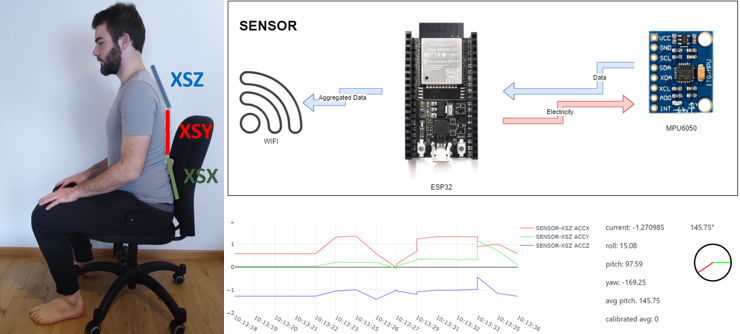
\includegraphics[width=\linewidth]{images/TitlePicture.png}
\end{textblock}

\begin{textblock}{154}(28,117)
	\begin{picture}(150,2)
		\put(0,0){\color{bfhgrey}\rule{150mm}{2mm}}
	\end{picture}
\end{textblock}
\color{black}

% Institution / titel / subtitel / authors / experts:
%---------------------------------------------------------------------------
\begin{flushleft}

\vspace*{115mm}

\fontsize{26pt}{28pt}\selectfont 
\heading				\\							% Read heading from file leader/title.tex
\vspace{2mm}

\fontsize{16pt}{20pt}\selectfont\vspace{0.3em}
A wearable IoT solution			\\				% Insert subheading
\vspace{5mm}

\fontsize{10pt}{12pt}\selectfont
\textbf{} \\		% Insert text
\vspace{3mm}

% Abstract (eingeben):
%---------------------------------------------------------------------------
\begin{textblock}{150}(28,190)
\fontsize{10pt}{12pt}\selectfont
Creating a prototype with modern IoT comoponents and topical knowhow to track and improve posture.
\end{textblock}

\begin{textblock}{150}(28,225)
\fontsize{10pt}{17pt}\selectfont
\begin{tabbing}
xxxxxxxxxxxxxxx\=xxxxxxxxxxxxxxxxxxxxxxxxxxxxxxxxxxxxxxxxxxxxxxx \kill
Authors:		\> Gabriel Frischknecht		\\					% insert names
Tutor:	\> Prof. Dr.~Reto Koenig		\\
Expert:	\> Prof. Dr.~Torsten Braun		\\% insert names
Date:			\> \versiondate					\\							% read from file leader/version.tex
\end{tabbing}

\end{textblock}
\end{flushleft}

\begin{textblock}{150}(28,280)
\noindent 
\color{bfhgrey}\fontsize{9pt}{10pt}\selectfont
Berner Fachhochschule | Haute \'ecole sp\'ecialis\'ee bernoise | Bern University of Applied Sciences
\color{black}\selectfont
\end{textblock}


\end{titlepage}

%
% ===========================================================================
% EOF
%
		% activate for frontpage with picture
% Control of versions :
% -----------------------------------------------

\begin{textblock}{180}(15,150)
\color{black}
\begin{huge}
Versions
\end{huge}
\vspace{10mm}

\fontsize{10pt}{18pt}\selectfont
\begin{tabbing}
xxxxxxxxxxx\=xxxxxxxxxxxxxxx\=xxxxxxxxxxxxxx\=xxxxxxxxxxxxxxxxxxxxxxxxxxxxxxxxxxxxxxxxxxxxxxx \kill
Version	\> Date	\> Status			\> Remarks		\\
1.0	\> 06.03.2019	\> Draft		\> First version with BFH	\\	
2.0	\> 06.05.2019	\> Draft		\> added technical basics	\\	
3.0	\> 06.06.2019	\> Draft		\> First final version	\\	

\end{tabbing}

\end{textblock}

\cleardoubleemptypage
\setcounter{page}{1}
\cleardoublepage
%---------------------------------------------------------------------------

% Table of contents
%---------------------------------------------------------------------------
\tableofcontents
\cleardoublepage
%---------------------------------------------------------------------------

% Main part:
%---------------------------------------------------------------------------
\pagenumbering{arabic}
\renewcommand\thefigure{\arabic{figure}}

\addcontentsline{toc}{chapter}{Introduction}
\chapter*{Introduction}
\label{chap:Introduction}
\renewcommand{\thesection}{\arabic{section}}
\setcounter{section}{0}

The long-term goal of this Project was first defined in 2017 and has been refined ever since. First and for most, the goal is to create a simple and cheap device(s) which can measure and improve posture. Additional it should all be open source and recreatable. Besides posture, the goal is also to offer a way to improve balance. 
With the idea of improving balance also comes a much larger goal which might not even be achievable. The solutions should be able to find application in the medicinal field, however this seams to be nearly impossible due to the complexity and restrictions in this field. 

Therefore I decided to split the long term goal into smaller steps which should be achievable one by one individually. During this thesis I will try to achieve the following:

Firstly I will need to find out how many Sensors are needed to get an understanding of the users Gait and Position. To Achieve this I will also need to find a way to visualise or interpret the data I am collecting.

\addcontentsline{toc}{chapter}{Technical Basics}
\chapter*{Technical Challenges}
\label{chap:Technical CHallenges}
\renewcommand{\thesection}{\arabic{section}}
\setcounter{section}{0}

The Goal of gathering and visualizing the data to define how many sensors are needed for useful evaluation leads to many different technical challenges. First an for most I will need to find a way to connect n sensors.


\section{Sensors and Data}

During my first 

\addcontentsline{toc}{chapter}{Results}
\chapter*{Results}
\label{chap:Results}
\setcounter{section}{0}

\addcontentsline{toc}{chapter}{Prospects}
\chapter*{Prospects}
\label{chap:Porspects}
\setcounter{section}{0}


\addcontentsline{toc}{chapter}{Conclusion}
\chapter*{Conclusion / Results}
\label{chap:Conclusion}

After more than semester of work, and finally a somewhat usable product, I am looking back at e few very intensive weeks and months. In hindsight, i realise, that my goals were ambitious and almost a bit to high for such a "small" project scope. I have achieved all my goals, but I suspect, my efforts exceed the planned, or credited effort in the "Project 2" module. 
Nonetheless I am very happy with what I have achieved and also do not regret setting the goals so high. The achievements give a great foundation for an interesting and diverse Bachelor Thesis, with a lot of potential.
Furthermore I have chosen a topic which I am highly interested in, which made the extra effort, very easy since it felt more like a hobby. Therefore I am looking forward to my last semester in my Bachelor degree and my bachelor thesis.

\cleardoublepage
\phantomsection 
\addcontentsline{toc}{chapter}{Declaration of authorship}
\chapter*{Declaration of primary authorship}
\label{chap:declaration_authorship}

\vspace*{10mm} 

I hereby confirm that I  have written this thesis independently and without using other sources and resources than those specified in the bibliography. All text passages which were not written by me are marked as quotations and provided with the exact indication of its origin. 

\vspace{15mm}

\begin{tabbing}
xxxxxxxxxxxxxxxxxxxxxxxxxxxxxx\=xxxxxxxxxxxxxxxxxxxxxxxxxxxxxx\=xxxxxxxxxxxxxxxxxxxxxxxxxxxxxx\kill
Place, Date:		\> Ostermundigen, \versiondate \\ \\ 
Last Name/s, First Name/s:	\> Gabriel Frischknecht 	 \\ \\ \\ \\ 
Signature/s:	\> ......................................\> \\
\end{tabbing}

%---------------------------------------------------------------------------

%---------------------------------------------------------------------------

% Bibliography
%---------------------------------------------------------------------------
\cleardoublepage
\phantomsection 
\addcontentsline{toc}{chapter}{Bibliography}
\bibliographystyle{IEEEtranS}
\bibliography{database/bibliography}{}
%---------------------------------------------------------------------------

% Listings
%---------------------------------------------------------------------------
\cleardoublepage
\phantomsection 
\addcontentsline{toc}{chapter}{List of figures}
\listoffigures
\end{document}

